\documentclass[11pt]{article}

\usepackage[ngerman]{babel}
\usepackage[T1]{fontenc}
\usepackage[utf8]{inputenc} 
\usepackage[pdftex]{graphicx}
\usepackage{pdfpages}
\usepackage{geometry,blindtext}

\geometry{a4paper,left=30mm,right=20mm, top=1cm, bottom=2cm, includeheadfoot}

\usepackage{float}

\usepackage{amsmath, amsthm, amssymb}

\usepackage[babel,german=quotes]{csquotes}


\usepackage{fancyhdr}
\pagestyle{fancy}
\fancyhf{}

\fancyfoot[L]{\small{\textbf{Basistechniken\\Miniprojekt Auslandssemester}}}

\fancyhead[L]{\small{David Brüggemann, Patrick Kotz, Merlin Fischer}}

\fancyhead[R]{\today}
\renewcommand{\footrulewidth}{0.4pt} %untere Trennlinie
\renewcommand{\headrulewidth}{0.4pt}

% Bei Problemen mit Umlauten:
% "uft8" durch "latin1", "ansinew" oder "applemac" ersetzen.

\begin{document}


\begin{titlepage}
  \title{Projektmanagment: \\Auslandssemester in Windhoek, Namibia}
  \author{Patrick Kotz, David Brüggemann, Merlin Fischer,\\ Fachhochschule Südwestfalen}
  \date{\today}
\end{titlepage}

\fancyfoot[C]{\thepage}

\maketitle

\newpage
\tableofcontents
\newpage

\section{Einleitung}
Ein Auslandsstudium bezeichnet einen Studienaufenthalt von meist ein bis zwei Semestern in einem anderen Land als dem, in dem das Studium aufgenommen wurde und normalerweise auch abgeschlossen werden kann.

\section{Projektauftrag}
Wir wollen ein Auslandssemester in der Universität Polytechnic of Namibia in Windhoek erfolgreich absolvieren und ohne große finanzielle Verluste zurückkehren.\\

Unter Erfolgreich absolvieren verstehen wir, dass alle Prüfungen an denen wir teilnehmen werden bestanden und anerkannt werden.\\

Unter finanziellen Verlusten verstehen wir, dass wir deutlich mehr in Namibia ausgeben als wir es zu hause tun würden. Um es Messbar zu machen nehmen wir unser Einkommen, welches bei 200-400 Euro liegt.

\newpage

\section{Projektplan}

\subsection{Zeitplan}
Ein dreiviertel Jahr bevor man das Auslandssemester beginnt, fangen die Vorbereitungen an. Man fängt damit an sich über die Termine für die Bewerbung zu informieren und eine Bewerbung auszufüllen. Innerhalb des Bewerbungszeitraums muss man diese dann nur noch abschicken. Zu dieser Zeit sollte man sich Impfen lassen, denn die Impfung sollte in einem Zeitraum von einem halben Jahr vor der Einreise in Namibia erfolgen. 

Direkt nachdem die Bewerbung angenommen wurde, beginnt der aufwendigste Teil der Vorbereitung. Zuerst muss man die Termine innerhalb des Semesters (Abgaben und Prüfungszeiträume) heraussuchen und dafür einen Terminplan erstellen.
Mithilfe dieses Terminplans kann man sich eine Unterkunft suchen und den Hin - und Rückflug buchen.  Außerdem muss ein Reisepass beantragt werden, falls man keinen besitzt. Dafür sollten drei bis vier Wochen eingeplant werden. Wenn diese Punkte erledigt wurden, sollte man anfangen die Anträge für ein Visum auszufüllen, um Stress am Flughafen zu vermeiden. Sind alle diese Punkte erfüllt steht einem nichts mehr im Weg ein Auslandssemester zu beginnen.

Ab dem diesem Zeitpunkt kann man sich auf das Lernen Konzentrieren und muss nur noch die Termine aus dem Terminplan einhalten und wichtige Dokumente bereithalten.

\begin{itemize}
\item Bewerbungstermine Herausfinden und Bewerbung ausfüllen (etwa ein 3/4 Jahr vorher)
\item Impfung					                           (etwa halbes Jahr vorher)
\item Bewerbung abschicken			(Anfang des Bewerbungszeitraums)
\item Termine des Semesters                                  ( )
\item Unterkunft suchen				(Nachdem man angenommen wurde)
\item Hin – und Rückflug buchen                           (Nachdem man angenommen wurde)
\item Reisepass beantragen[falls nötig]		(Bearbeitungszeit von drei bis vier wochen)
\item Anträge (Visum)				(Kurz vor dem Hinflug [am besten Frühzeitig])
\item Hinflug
\item Termine im Semester (Prüfung etc.)
\item Rückflug

\end{itemize}
Informationen zum Reisepass:
http://www.fremdenverkehrsbuero.info/reisepass-beantragen.php

\newpage

\subsection{Kosten}
Kosten gering halten:
Förderung: „go to Afrika“ (zur Zeit Abgelaufen)
Auslands bafög beantragen
Stipendien
Jobs vor Ort (Eventuell schwer zu finden)\\

Ausgabenquellen:\\
Flug (ungefähr 1000 Euro mit Air Berlin)siehe Anhang\\
Versicherung (Reiseversicherung oder Privatversicherung)\\
Unterkunft (300-400 Euro im Monat )\\
Semester gebühren (Entfällt bei uns)\\
30 Euro Bearbeitungsgebühr für einen Antrag auf ein befristetes Studium und ca 40-140 Euro für die Studienzeit

Fix Kosten 		ungefähr 1000 Euro
			400 Euro pro Monat

variable Kosten 	200 Euro pro Monat\\

Die Preise für Lebensmittel, Kleidung und ähnliches sind vergleichbar mit Deutschland

\subsection{Vorkehrungen}

\subsubsection{Impfung}
Es wurde ärztlich empfohlen ein Impfschutz gegen:
\begin{itemize}
\item Diphtherie
\item Tetanus
\item Polio,
\item Hepatitis A
\item Masern (oder Immunität nach Krankheit)
\end{itemize}
machen zu lassen und zwar ca ein halbes Jahr vor der 
Abreise. \\\\
Für Risikogruppen zusätzlich die Impfung gegen:
\begin{itemize}
\item Hepatitis B
\item Tollwut
\item Meningokokken
\item Pneumokokken
\item Influenza
\end{itemize}
 machen zu lassen. Dies ist aber sehr individuell und muss mit dem eigenen Hausarzt besprochen werden.
\\
Windhoek und Süd-Namibia sind Malariafrei, daher müssen diesbezüglich keine Vorkehrungen getroffen werden. 
\\
Ein Impfzertifikat ist beim Arzt einzufordern und muss unter umständen am Flughafen in Windhoek vorgezeigt werden.

\subsubsection{Anträge}
Anträge zum Studium für das Visum und Arbeitserlaubnis sollten vorher rausgesucht werden und möglichst ein halbes Jahr vor der Abreise bei dem entsprechenden Amt eingereicht werden. Verschiedene Anträge befinden sich im Anhang zum ausfüllen bereit.

\subsection{Flug}
Zeit zum Einplanen des Fluges: Der Flug dauert in der Regel ca 10-15 Std auf die man sich einstellen sollte.
Siehe dazu Anhang

\newpage

\section{Reflexion Einzelansicht}
\subsection{Patrick Kotz}
\subsubsection{Einstellung zum Projekt}

Das Thema des Projektes ist die Planung eines Auslandssemester oder Praxissemester. Das Thema Praxissemester war nicht von Interesse für mich, da ich denke, dass man nach dem Studium sein ganzes Leben lang Zeit Erfahrungen in der Arbeit zu sammeln. Ein Auslandssemester dagegen bietet die Möglichkeit in ein anderes Land zu reisen, die zwischenmenschliche  Kommunikation zu verbessern, sowie Sprachkenntnisse zu steigern und neue Leute kennen zu lernen und deshalb ich habe mich dann für das Auslandssemester entschieden. 



\subsubsection{Gruppe}

Die Bearbeitung des Projekts innerhalb der Gruppe verlief sehr gut. Es gab keine Streitigkeiten innerhalb der Gruppe und falls Gruppenmitglieder unterschiedlicher Meinung waren, hat sich die Gruppe einigen können. Ich denke die Arbeit war gerecht aufgeteilt, sodass kein Gruppenmitglied sich benachteiligt fühlen musste. Die Motivation war bei allen kontinuierlich hoch. Das konnte man anhand der mit Interesse verfolgten Bearbeitung erkennen. Niemand hat es nur als Pflichtprojekt angesehen.\\\\
Dass es innerhalb von Projekten kleinere Probleme gibt ist selbstverständlich, jedoch fällt mir zu diesem Projekt nur ein, dass einige Termine nicht eingehalten wurden, weil wir uns in diesem Punkt nicht gründlich abgesprochen hatten. Bestimmt ist jedem Gruppenmitglied dies Bewusst und jeder wird in zukünftigen Projekten daran denken.



\subsubsection{Fazit aus dem Projekt}

Ich kann nicht behaupten dieses Projekt hätte mir sehr viel gebracht. Ich kann die Unterlagen dazu verwenden ein Auslandssemester zu planen, aber im Moment verspüre ich nicht den Drang ein Auslandssemester durchzuführen.  \\
Dieses Projekt diente nicht dazu Wissen über ein bestimmtes Land aufzubauen oder Wissen über ein Auslandssemester zu vermitteln, auch wenn dies zweifellos ein Grund für die Themenvorgabe war. Das Ziel war ein Projekt durchzuführen und uns auf wichtige zukünftige Projekte vorzubereiten. Ich denke nicht, dass ich nach Abschluss dieses Projekts andere Projekte erkennbar besser durchführen kann als ich es vorher gekonnt hätte.\\
Das soll nicht heißen ich hätte nichts gelernt. Ich bin sicherer im richtigen Umgang mit Gruppenmitgliedern und der Zeiteinteilung geworden. So werde ich in zukünftigen Projekten fordern, dass wir uns Gedanken darüber machen zu welchen Zeitpunkten unser Projekt einen bestimmten Fortschritt erreichen soll. Ich werde dringender darauf bestehen Termine für das Projekt zu vereinbaren und ich werde vorschlagen Kontaktdaten zu Beginn des Projekts auszutauschen, damit jedes Gruppenmitglied erreicht und informiert werden kann.

\subsection{David Brüggemann}
\subsubsection{Einstellung zum Projekt}
Das Projekt Auslandssemester war für mich durchaus interessanter als das Praxissemester, da ich finde das im Praxissemester man nur Zeit verliert und ich mir vorgenommen habe das Studium möglichst schnell durchzuziehen. \\ Das Auslandssemester dagegen bietet Möglichkeiten andere Länder und Sitten kennenzulernen, wie man so schön sagt. Somit auch mal ganz andere Erfahrungen bekommt die man nicht in einem Urlaub oder ähnliches bekommt. Hier muss man auch mit Studenten und Professoren aus anderen Ländern arbeiten und das in anderer Sprache und Gewohnheiten.
\subsubsection{Meinung zur Gruppe}
Die Gruppe mit der ich das Projekt bearbeiten durfte gefiel mir gut. Es gab wenig bis keine Meinungsverschiedenheiten bei Arbeitsteilungen. Jeder wusste zu jeder Zeit wie der Stand des Projektes ist und was im nächsten Schritt getan werden muss. Die Motivation war nicht immer herausragend, jedoch wurde in jeder Sitzung das zuvor besprochene Ziel erreicht, was wie ich finde eine gute Zusammenarbeit ausmacht. Ab und zu hat es am Zeitmanagement gehackt allerdings lag das an falsch interpretierten Absprachen und hat sich letztendlich nicht auf die Gruppe ausgewirkt. Kritik und Vorschläge wurden von allen geäußert und gut ausgenommen.
\\ Zusammenfassend finde ich war ich mit der Arbeit der Gruppe und den Mitgliedern voll zufrieden.

\subsubsection{Fazit}
Es ist nicht so als hätte ich nach dem Projekt einen größeren Drang ein Auslandssemester zu machen. Nach meiner Meinung ist der Aufwand so ein Projekt zu planen auch zu aufwändig und hat mehr Zeit in Anspruch genommen als das vorgegebene Maximalbudget es zuließ. Allerdings war es auch mal ganz gut zu dritt an einem Projekt/Dokument zu arbeiten um nachher einen Bericht vorlegen zu können an denen alle ihren Teil beigetragen haben.

\subsection{Merlin Fischer}
\subsubsection{Einstellung zum Projekt}

Das Thema "`Studieren in Namibia"', als Auslandssemester, haben ich aus Interesse gewählt, da ich eine solches Semester gerne einmal machen würde, aber auch, da ein Praxissemester für mich nicht von Interesse ist, da ich gerne meine Sprachfähigkeiten verbessern möchte.
Da ein Auslandssemester genau das bietet, habe ich mich entschlossen ein solches Thema als Projektthema zu wählen.

\subsubsection{Gruppe}

Die Projektbearbeitung verlief, meiner Ansicht nach, sehr gut, obwohl es zwischendurch zu dem einen oder anderem Fauxpas in Sachen Terminabsprache gekommen ist.\\
Streitigkeiten oder ähnliches, sind in unserer Gruppe nicht aufgetreten, sowie auch keine Benachteiligung in der Bearbeitung innerhalb unseres Projekts.\\
Die Motivation war, aus meiner Sicht, bei allen kontinuierlich auf einem sehr hohen Level, wobei meine sich eher aus dem Interesse am Thema herleiten lässt.
\\\\
Weiter Probleme, außer in Hinsicht auf die Termine, hatten wir in unserer Gruppe keine.\\
Ich werde, für zukünftige Projekte, darauf achten, dass die Absprachen in dem Bereich Termine deutlich besser gehandhabt werden und wenn nötig auch an dieser Stelle selbst die Initiative ergreifen.

\subsubsection{Fazit}

Die Gruppenarbeit an sich, hat mir, denke ich, bis auf den kleinen Fauxpas, nicht viel gebracht, da Gruppenarbeiten bzw. -projekte nichts neues für mich sind.\\
Trotzdem war es einmal gut zu sehen, was auf einen zukommt, wenn man tatsächlich ein Auslandssemester plant bzw. bestreiten möchte.
Ob ich nun wirklich ein Auslandssemester absolvieren werde, kann ich noch nicht sagen, aber wenn ich die Möglichkeit habe, werde ich es machen.

\newpage

\section{Reflexion zum Projektverlauf aus Gruppensicht}
Das Thema "`Studieren in Namibia"' , als Auslandssemester, haben wir, unter anderem, 
aus Interesse gewählt, aber auch, weil ein Praxissemester hierzulande für uns nicht 
in Frage kommt, da wir gerne unsere Sprachfähigkeiten erweitern und verbessern wollen.
\\\\
Unsere Erwartung an das Thema "`Studieren in Namibia"' waren, dass wir vorab schon mal
wissen was auf uns zukommt, wenn wir ein Auslandssemester machen wollen, auch
wenn wir letztendlich vielleicht nicht in Namibia studieren.
\\\\
Das Ergebnis unserer Gruppenarbeit orientiert sich wesentlich an unseren Erwartungen,
aber natürlich auch an den Vorgaben und verbesserte sich durch das persönliche Interesse
an dem Thema "`Studieren in Namibia"' im Rahmen eines Auslandssemesters.
\\\\
Die Gruppenarbeit ist, geleitet von unserem eigenen Interesse an einem Auslandssemester,
kontinuierlich positiv verlaufen, da die Aufgabenteilung, sowie die Zusammenarbeit
unter- und miteinander gut funktioniert hat.
Informationen ließen sich teilweise sehr schwer konkret herauszufinden.
Zum Beispiel: "`Wie teuer ist ein Flug?"' lässt sich nur ungefähr beantworten.
\\\\
Probleme bei der Zusammenarbeit innerhalb der Gruppe gab es keine, aber die 
Terminabsprache lief zwischendurch nicht optimal.
\\\\
Aufgrund unseres Interesses, war die Motivation an dem Thema nicht schwer zu halten
und die Arbeitsleistung leicht zu bringen, die erwartet wurde.

\newpage

\section{Anhang}
\subsection{Stakeholder Liste}
\begin{itemize}
\item Familie
\item Freunde
\item Vermieter
	\\-Hier
	\\-In Namibia
\item Professoren
	\\-Hier
	\\-In Namibia
\item Stipendien
\item ehemalige Studenten
\item Fluggesellschaft
\end{itemize}

\subsection{Anmerkungen zu Berichten und Protokollen}
Die Statusberichte wurden in das Fach von Herrn Hühne geworden und wir haben dummerweise keine Kopie davon angefertigt. Wir bitten dies zu entschuldigen.
\\
Sitzungsprotokolle wurden nicht geführt sondern nach jeder Sitzung, wenn nötig, der Statusbericht angefertigt.

\subsection{Sonstiger Anhang}
\begin{enumerate}
\item Antrag auf Studium
\item Anträge auf Arbeitsplatz
\item Gesundheitsbefund
\item Radiologisches Gutachten
\item Bewerbung für das Studium an der Polytec
\item Screenshots zum Flug
\end{enumerate}

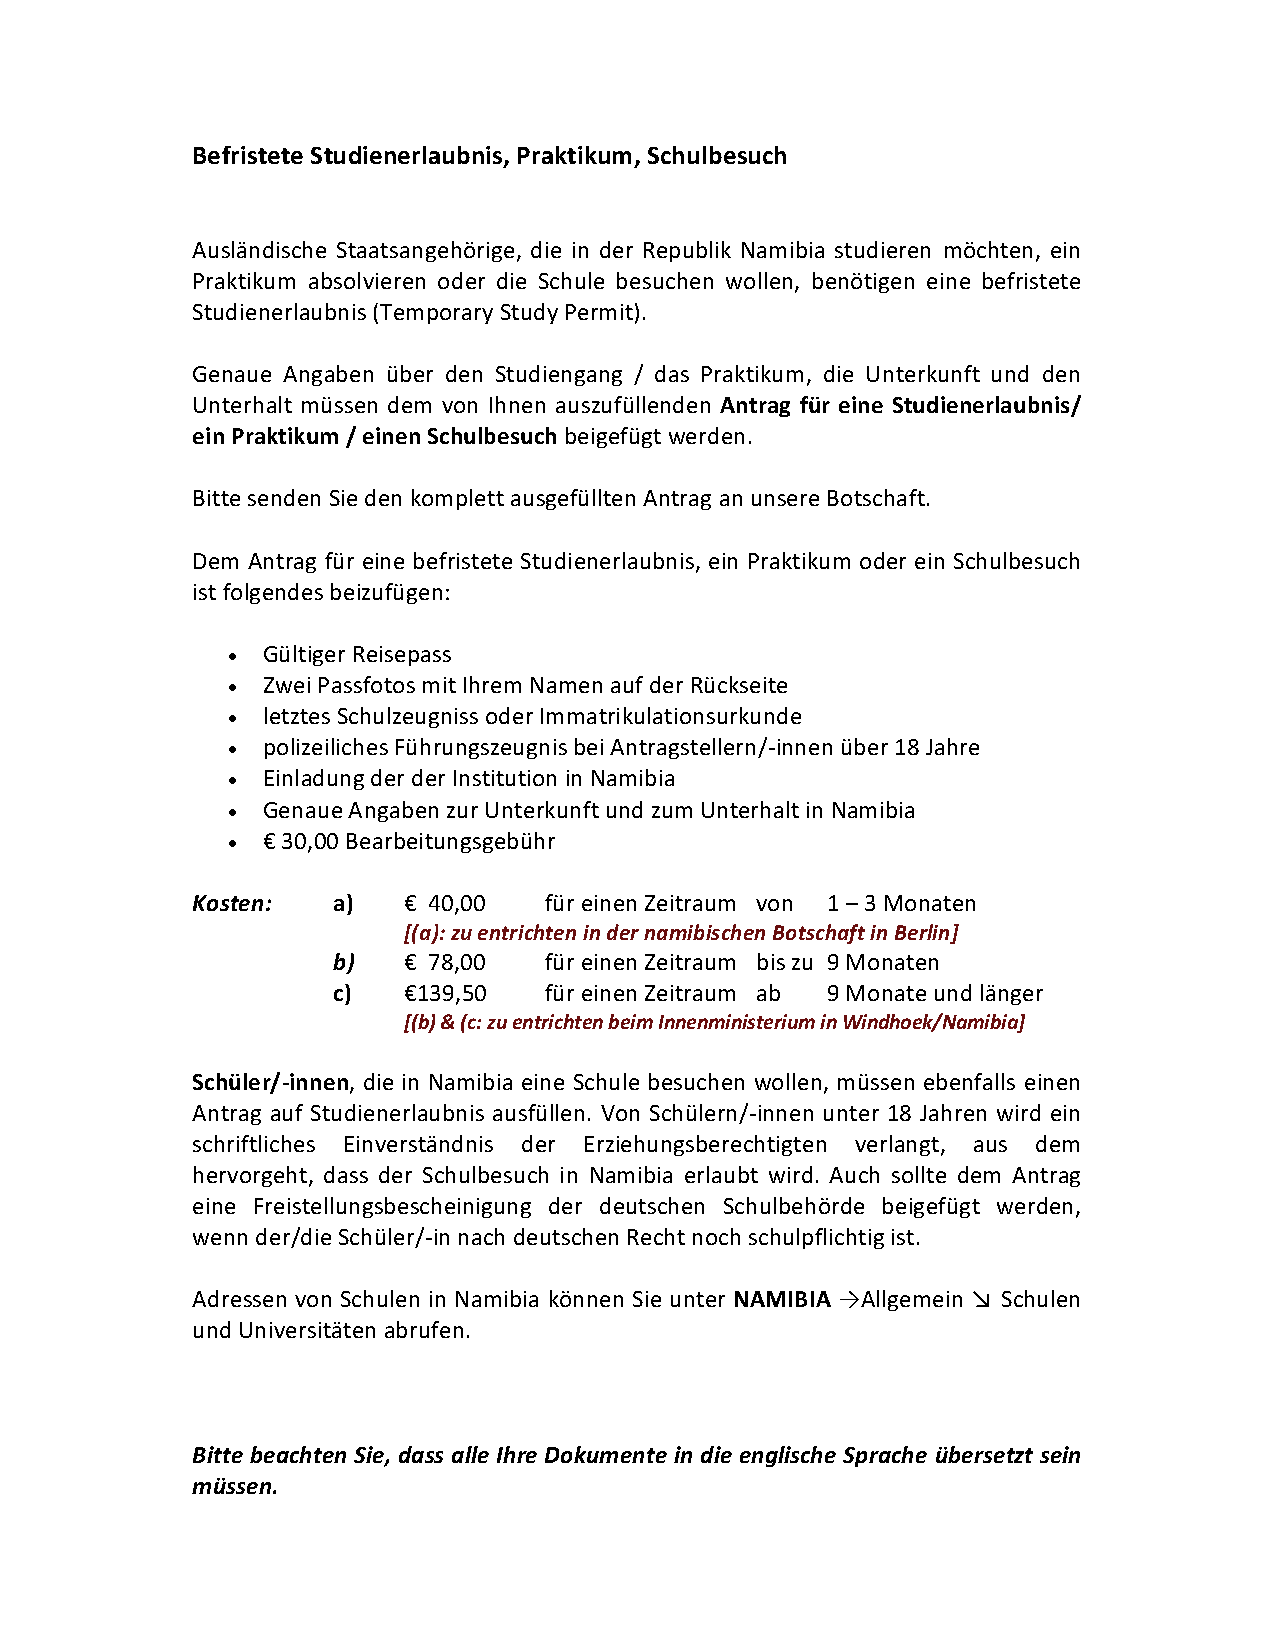
\includepdf[pagecommand={\thispagestyle{fancy}},noautoscale ,scale=0.9,pages=-]{merkblatt_befristete_studienerlaubnis.pdf}

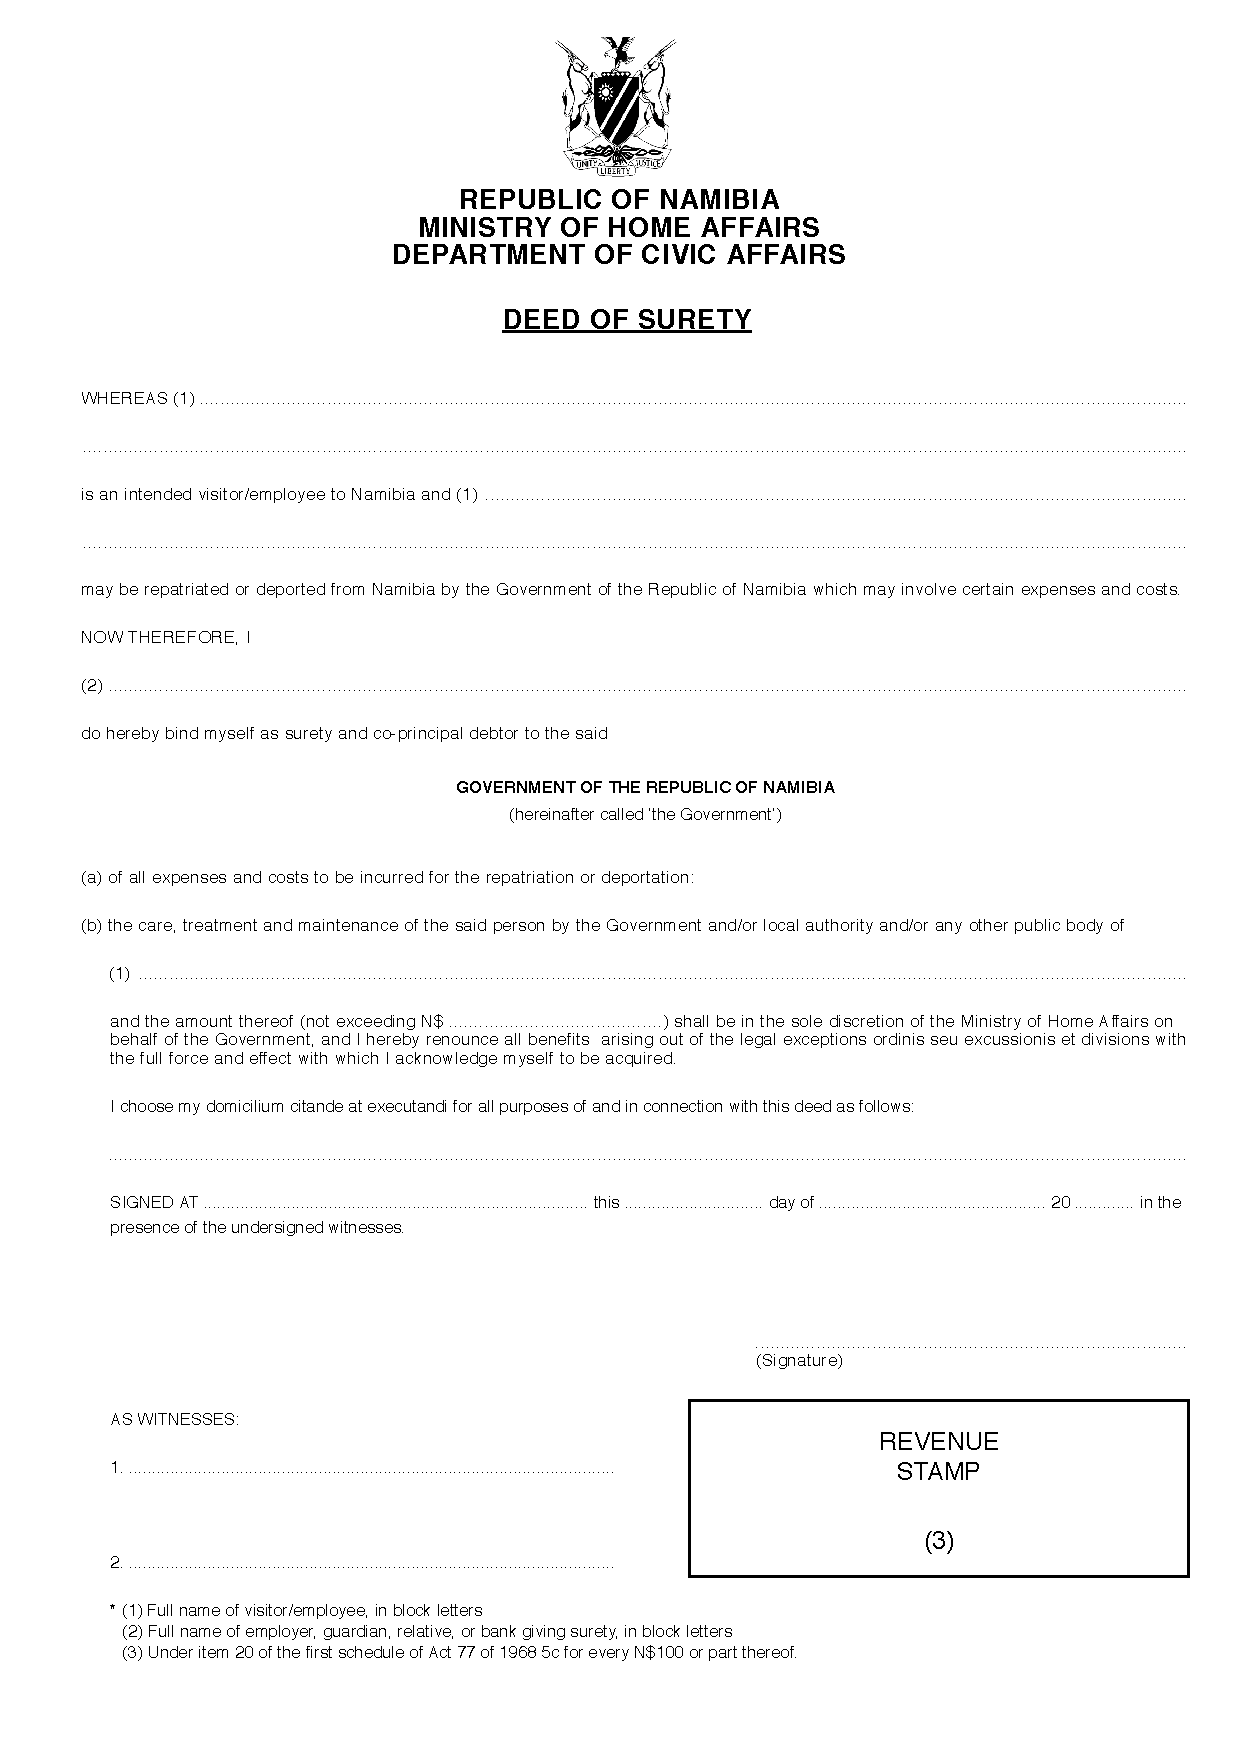
\includepdf[pagecommand={\thispagestyle{fancy}},noautoscale ,scale=0.9,pages=-]{Arbeitserlaubnis/deed_of_surety.pdf}

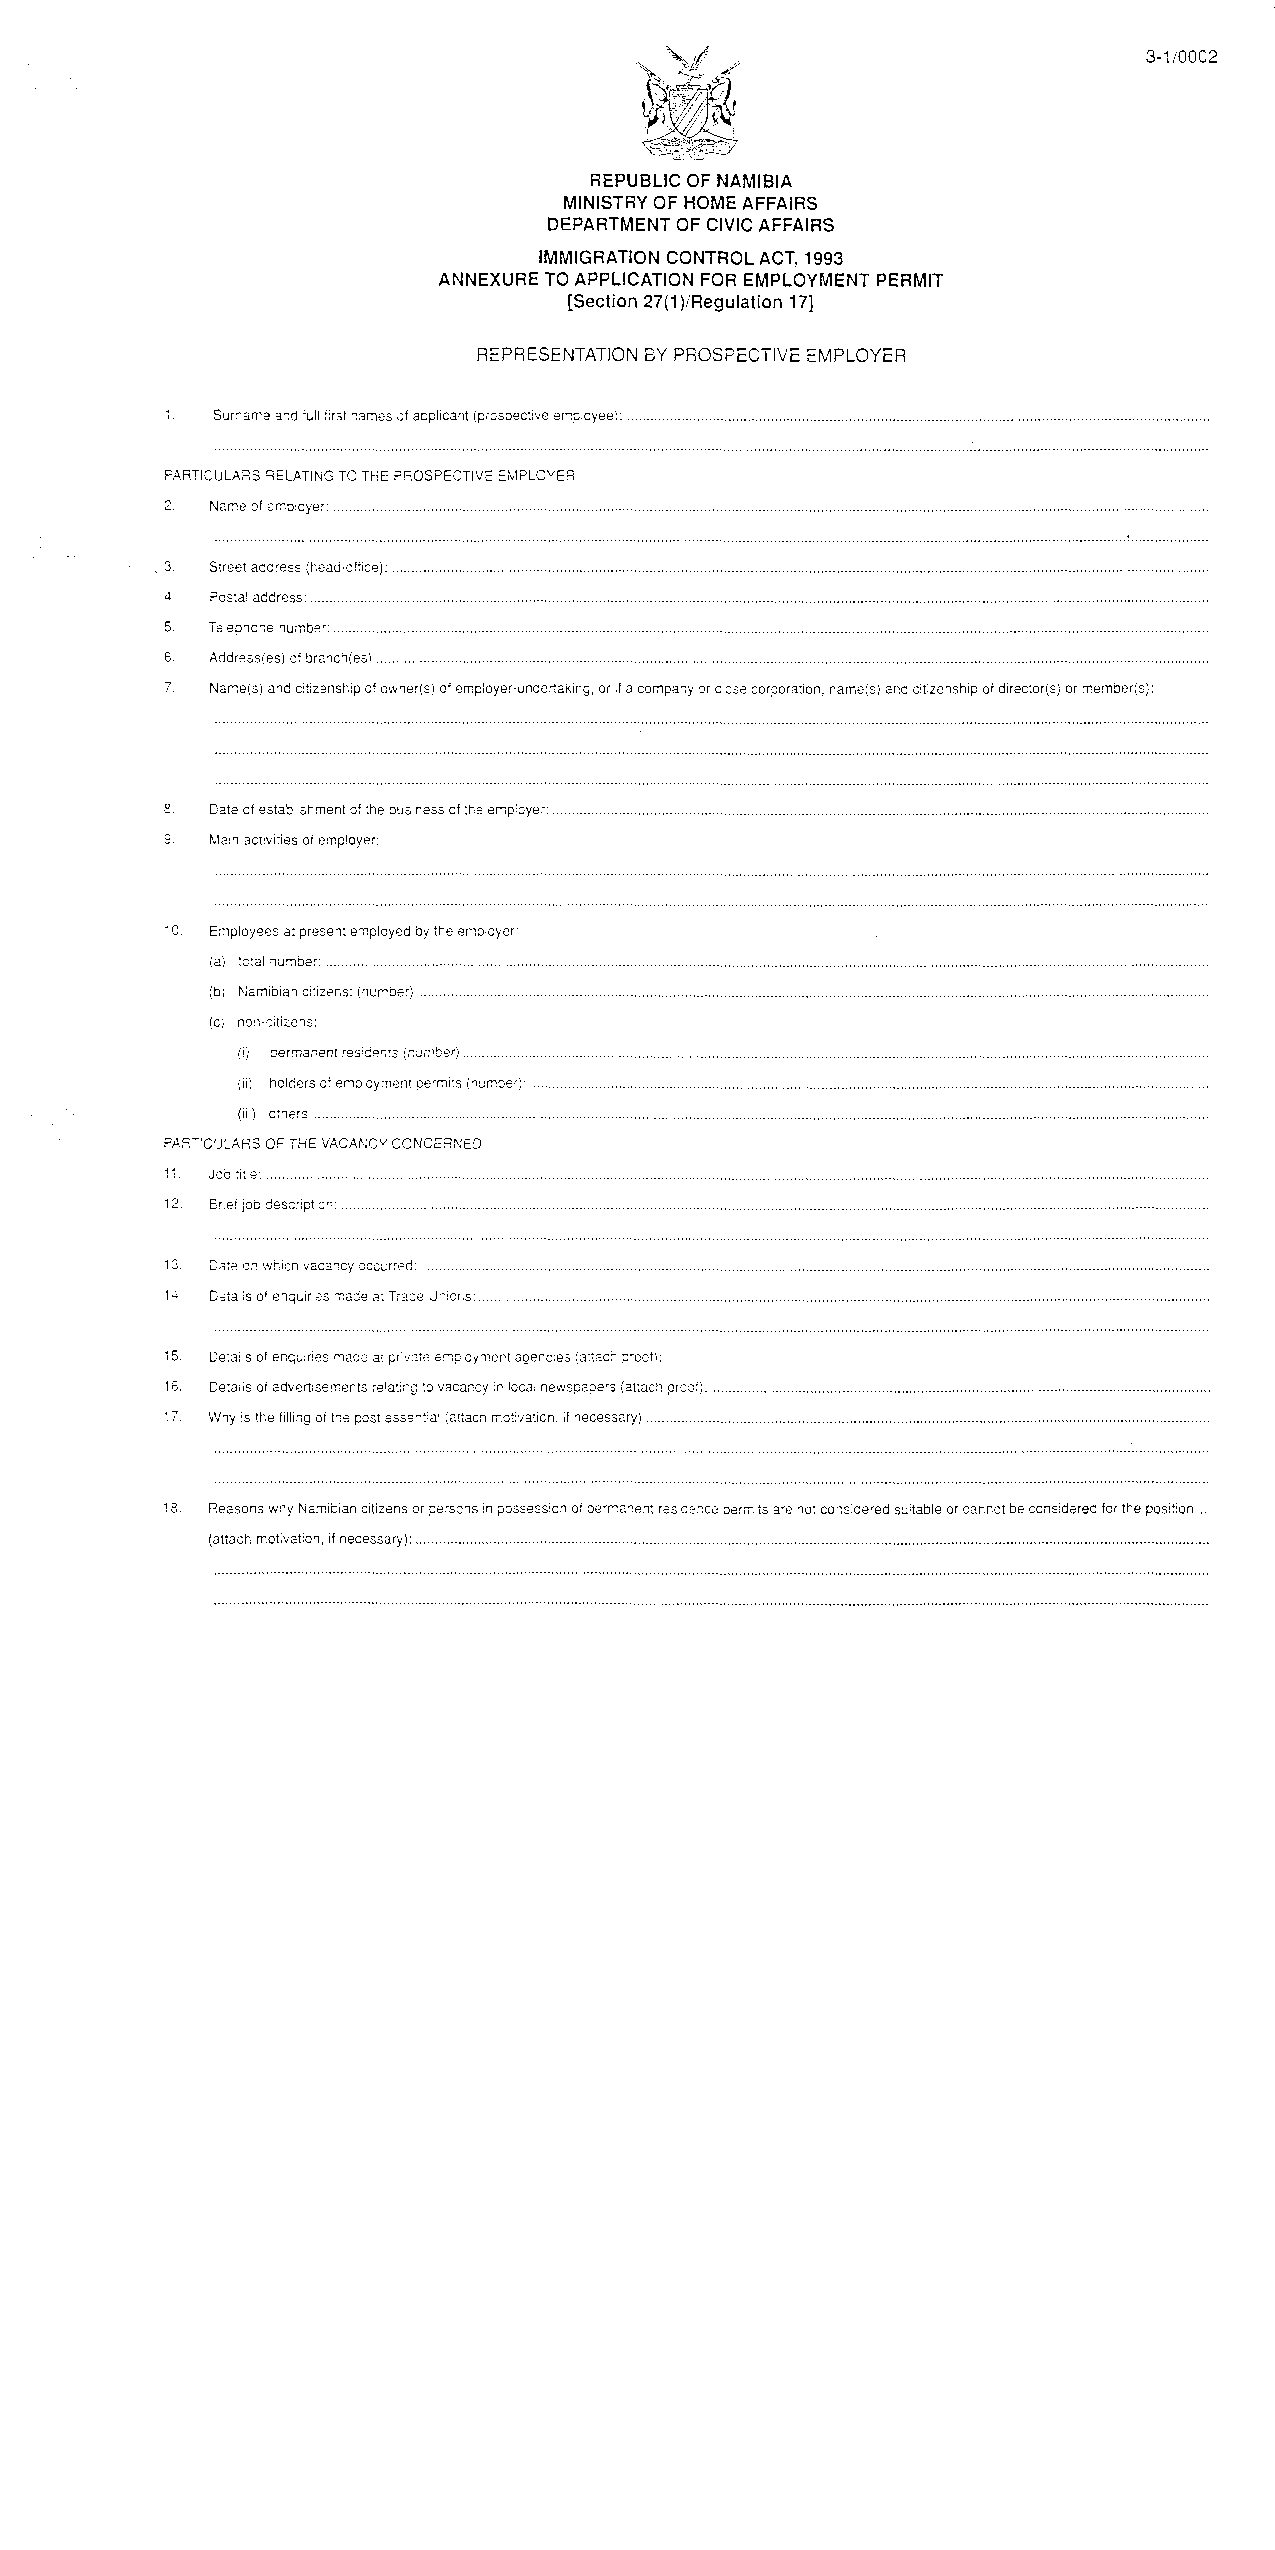
\includepdf[pagecommand={\thispagestyle{fancy}},noautoscale ,scale=0.9,pages=-]{Arbeitserlaubnis/prospective_employer_1.pdf}

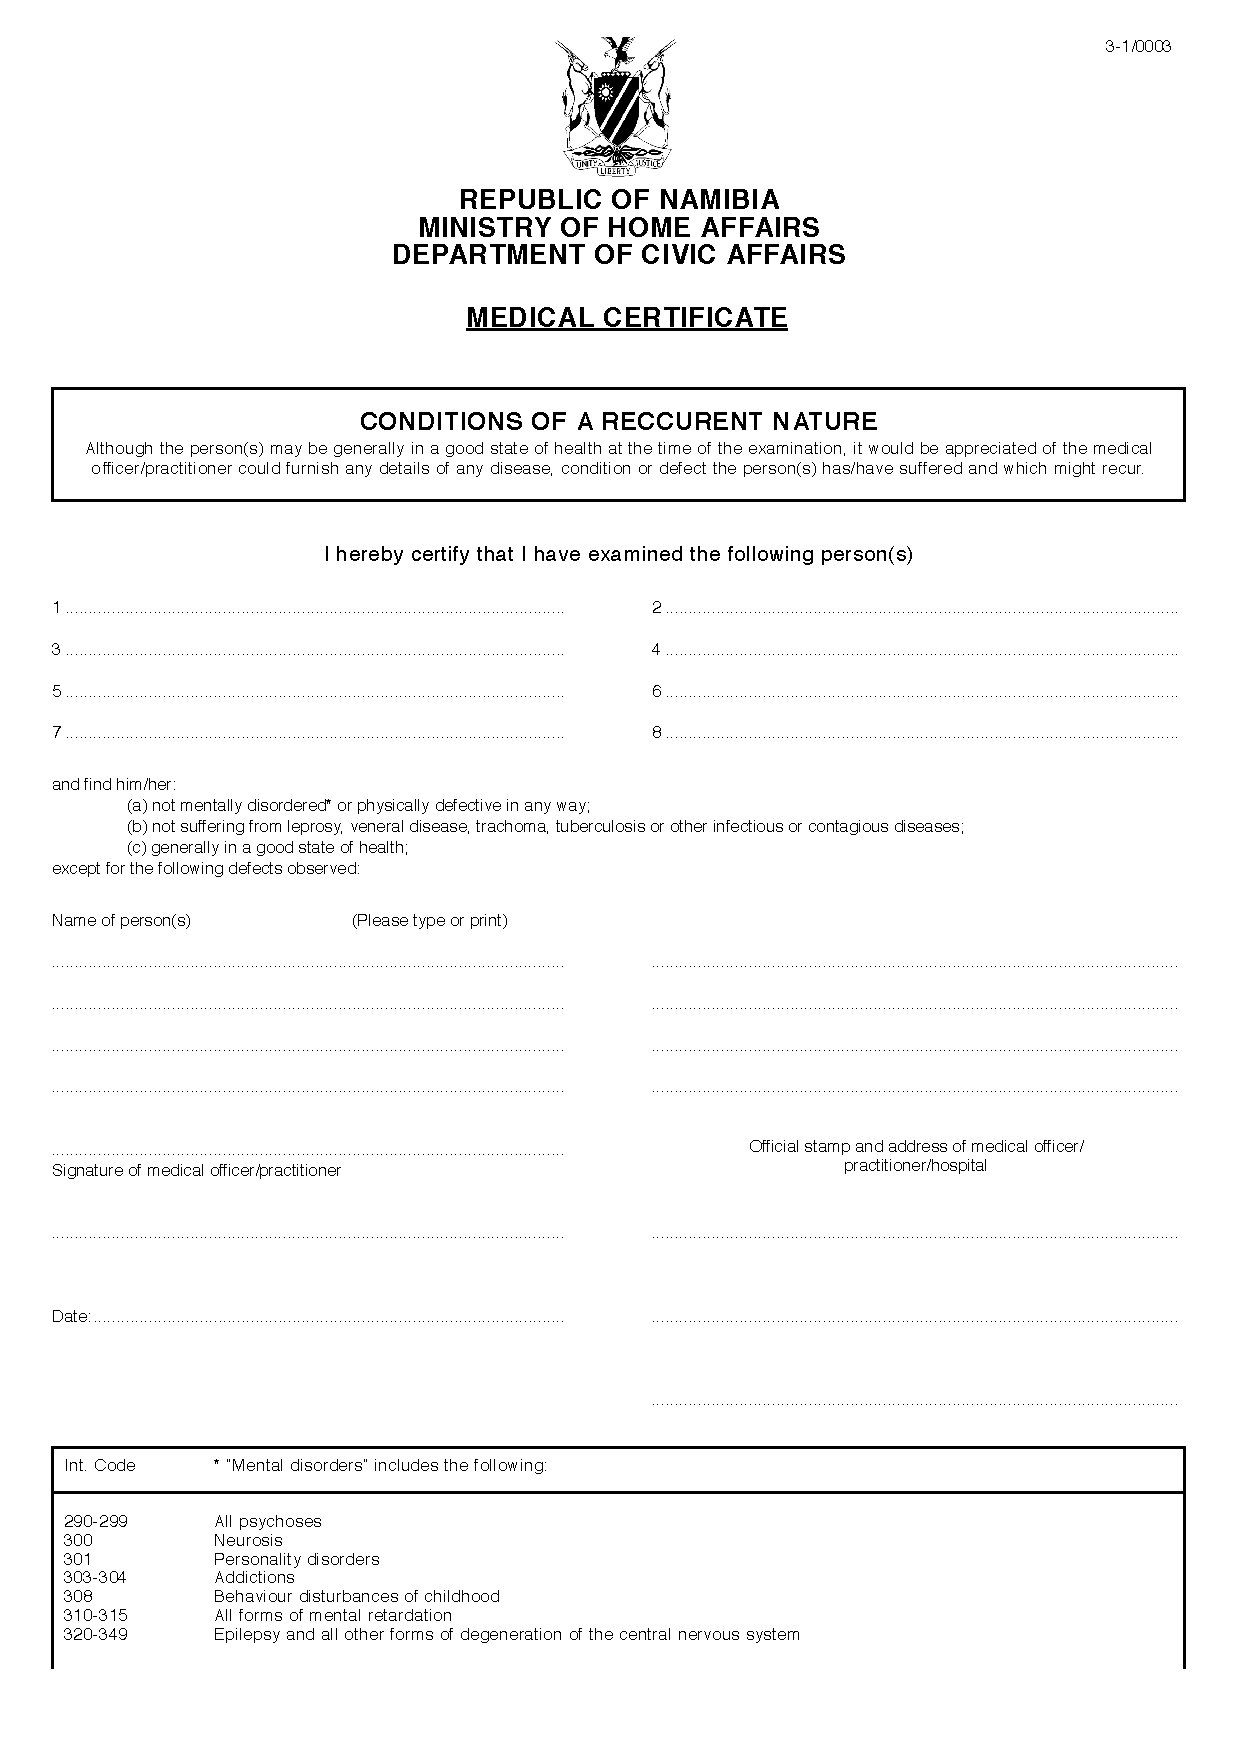
\includepdf[pagecommand={\thispagestyle{fancy}},noautoscale ,scale=0.9,pages=-]{Visum/Antrag_medical.pdf}

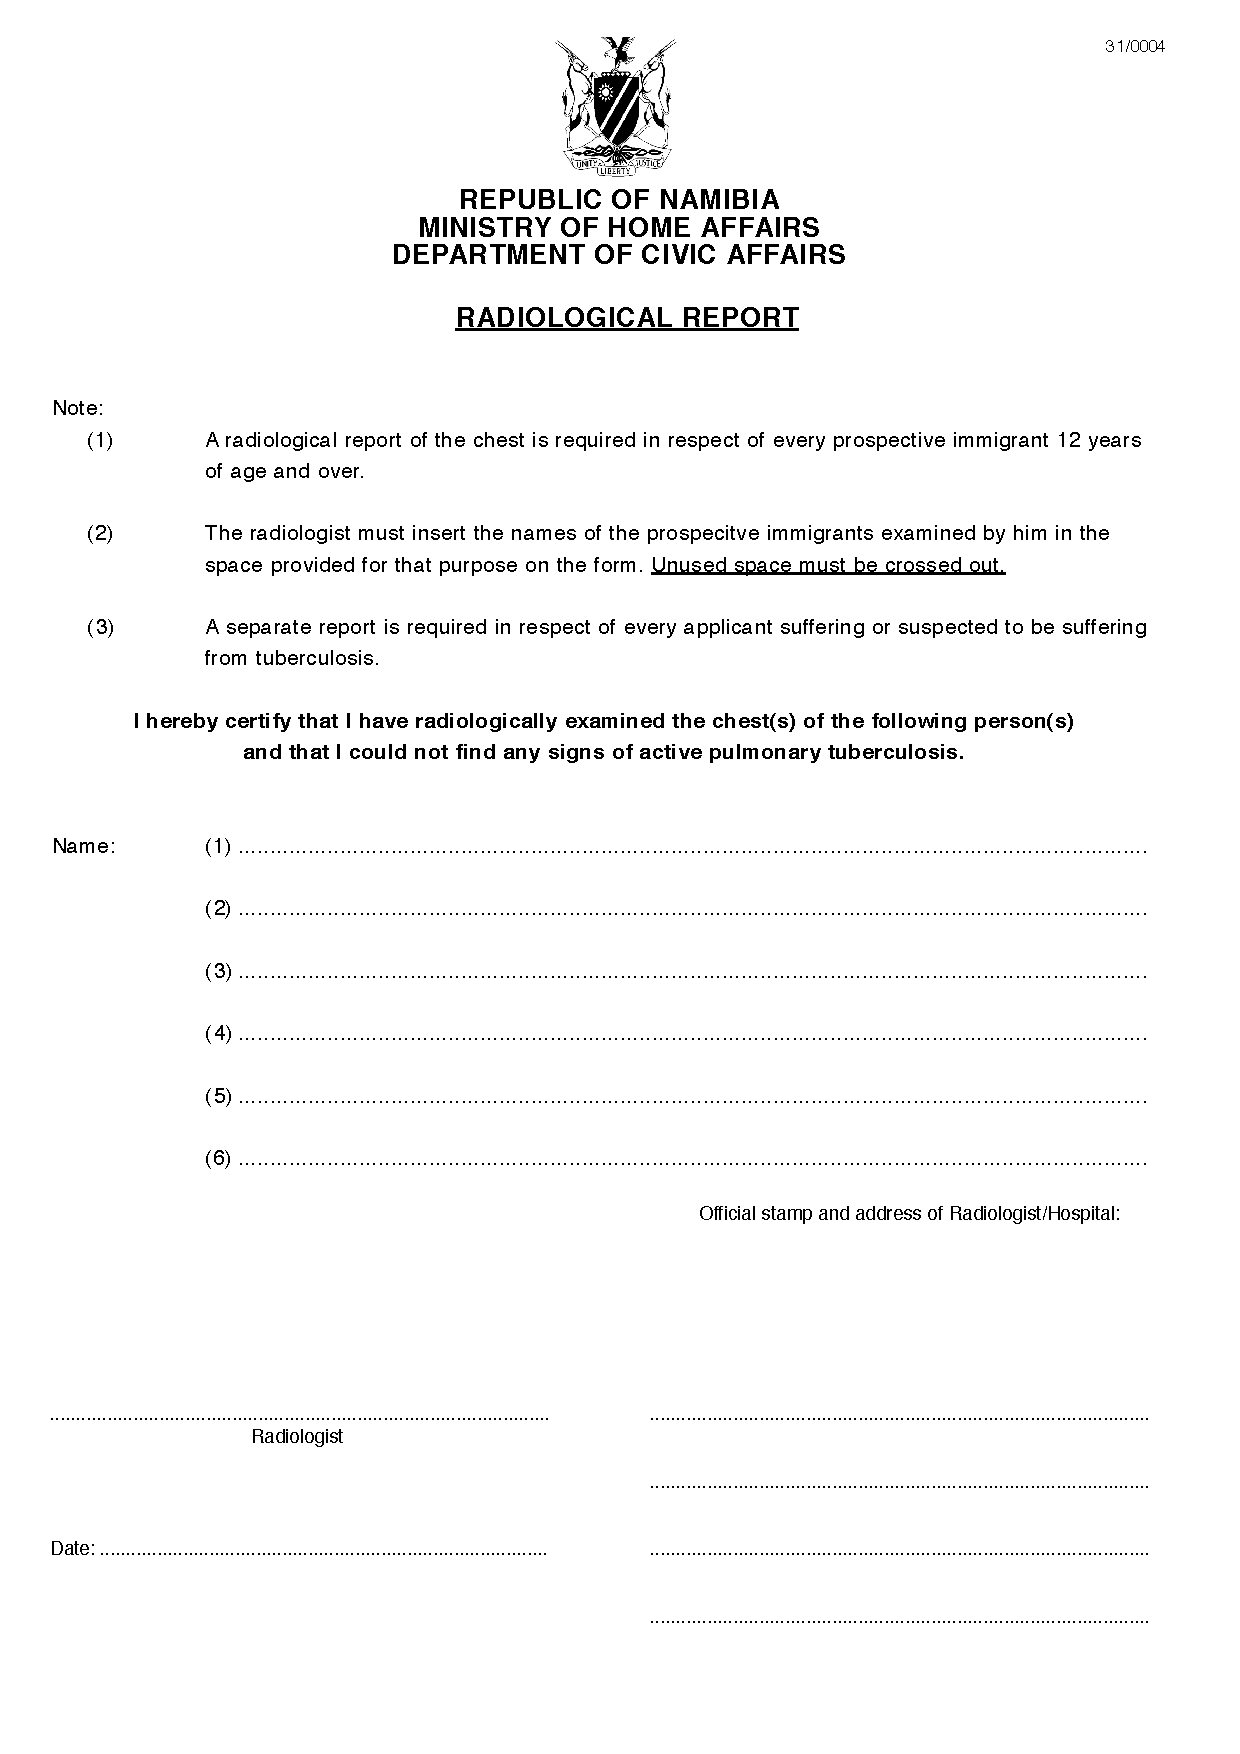
\includepdf[pagecommand={\thispagestyle{fancy}},noautoscale ,scale=0.9,pages=-]{Visum/Antrag_radiological.pdf}

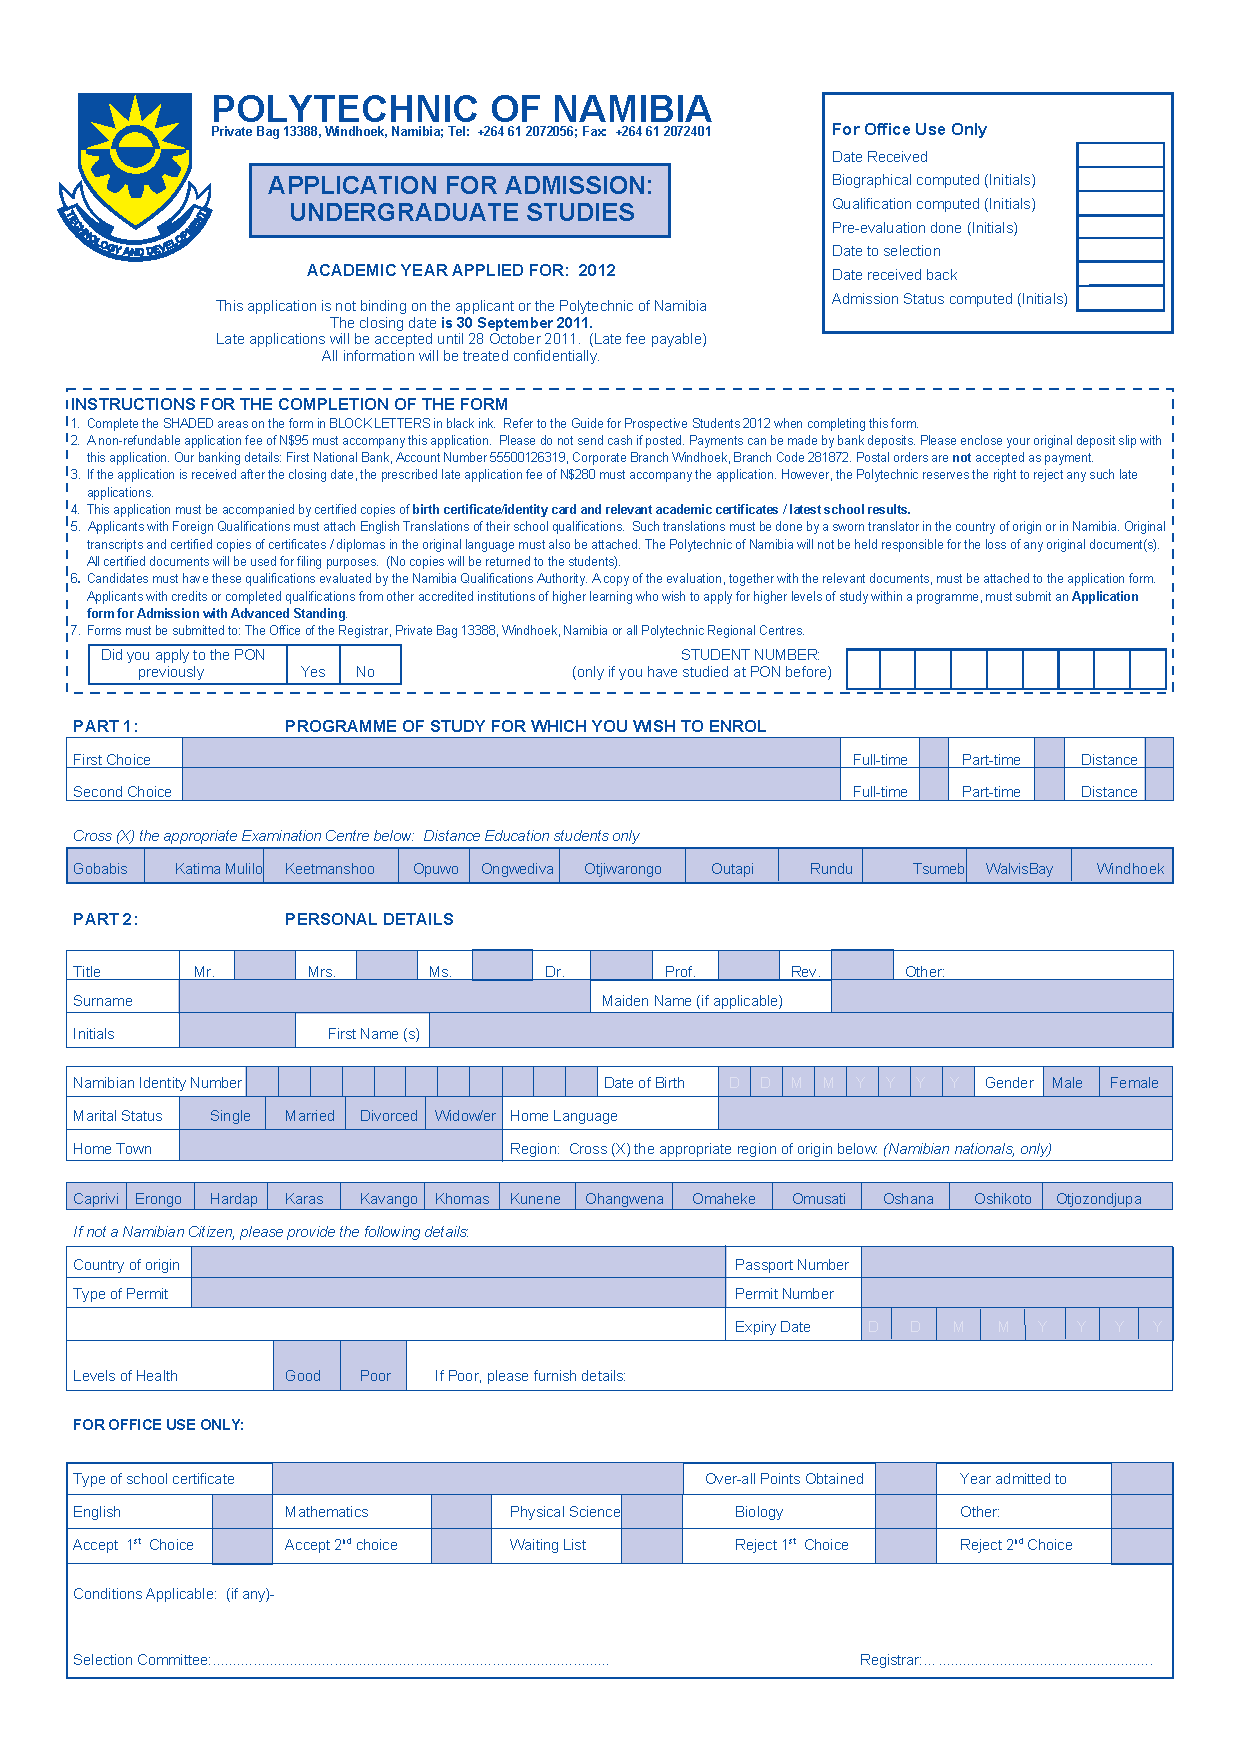
\includepdf[pagecommand={\thispagestyle{fancy}},noautoscale ,scale=0.9,pages=-]{Bewerbung_Schule/app_form.pdf}

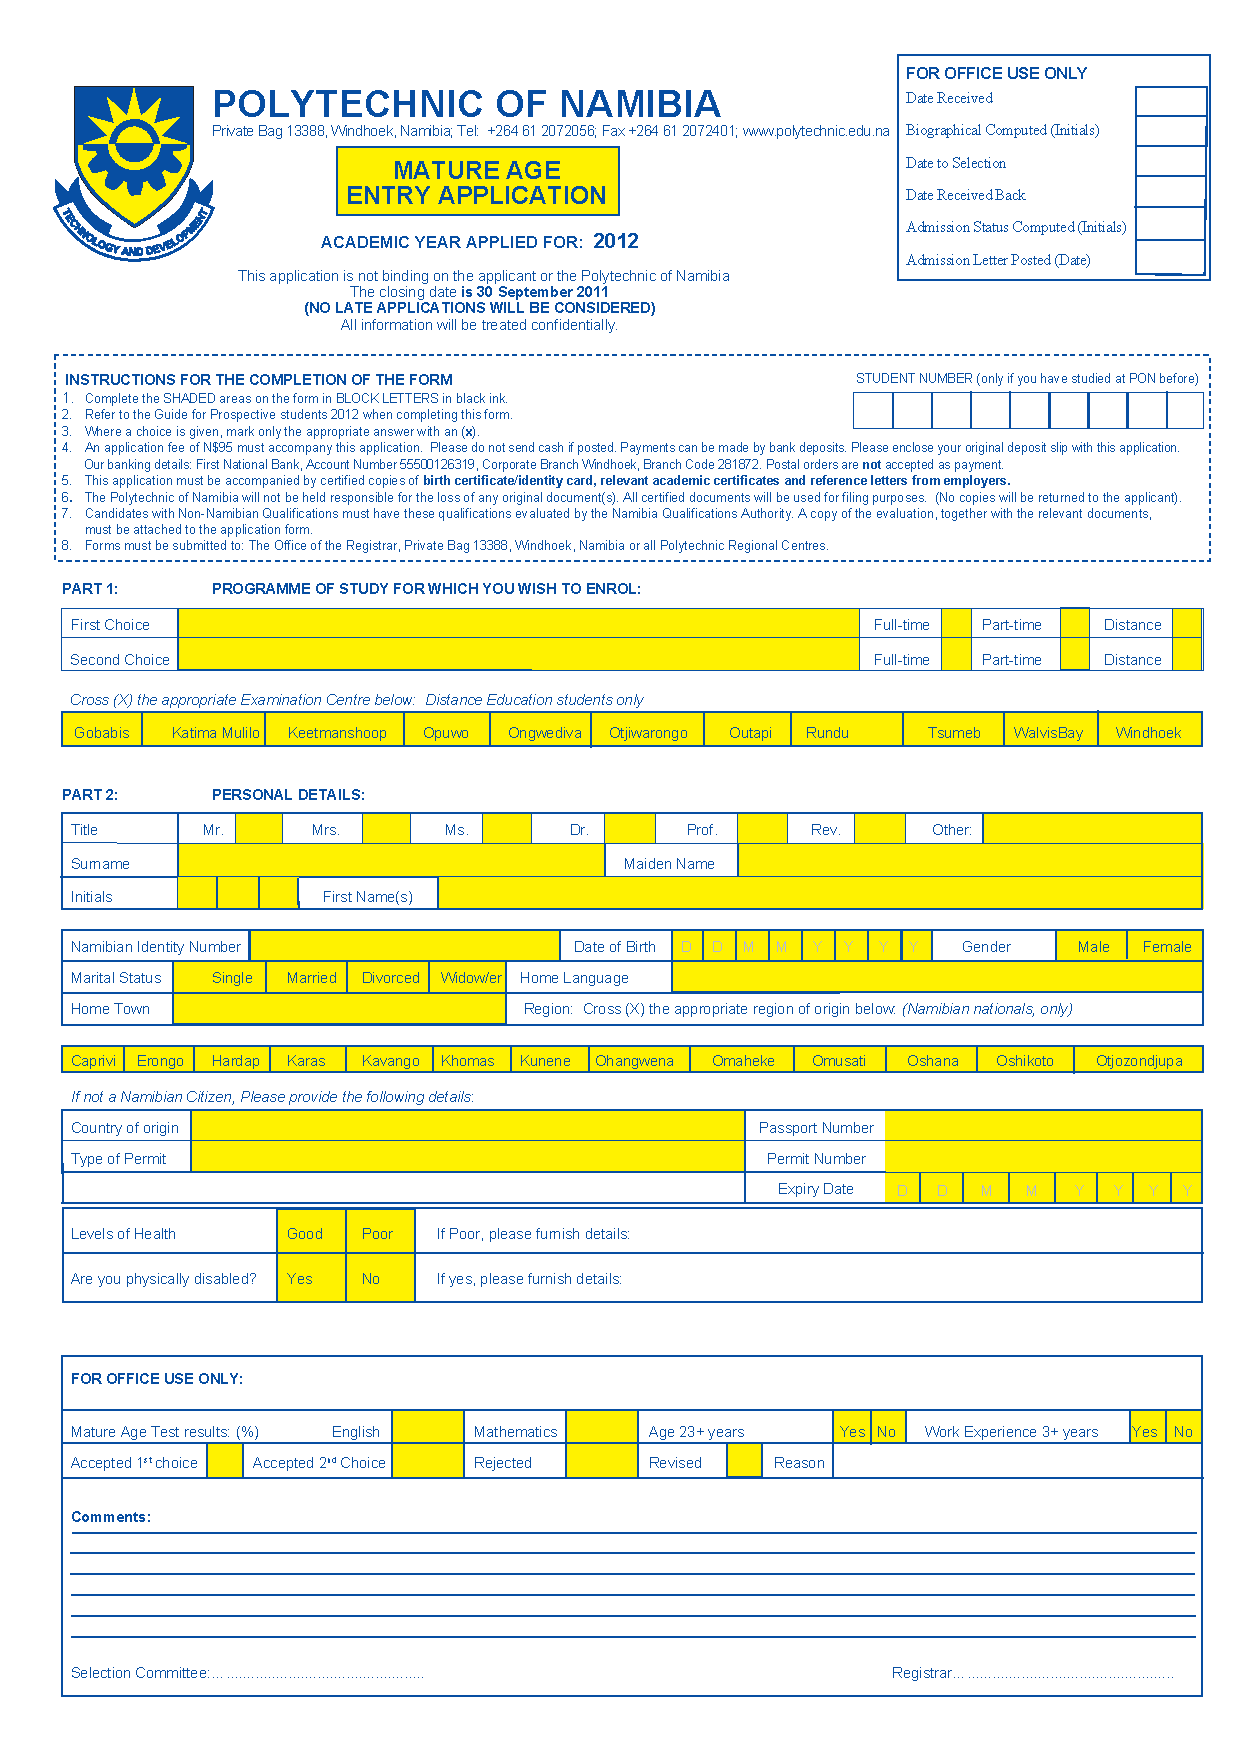
\includepdf[pagecommand={\thispagestyle{fancy}},noautoscale ,scale=0.9,pages=-]{Bewerbung_Schule/app_mature.pdf}

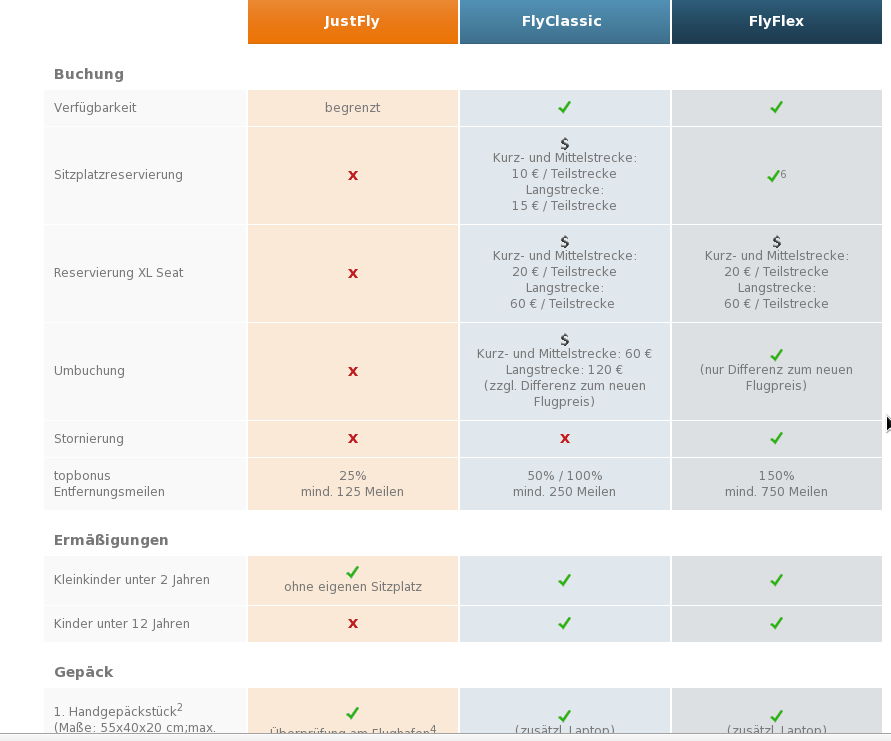
\includegraphics[scale=0.45]{Flug_Air_Berlin/Bildschirmfoto_am_2012-06-13_14_47_20.png} 

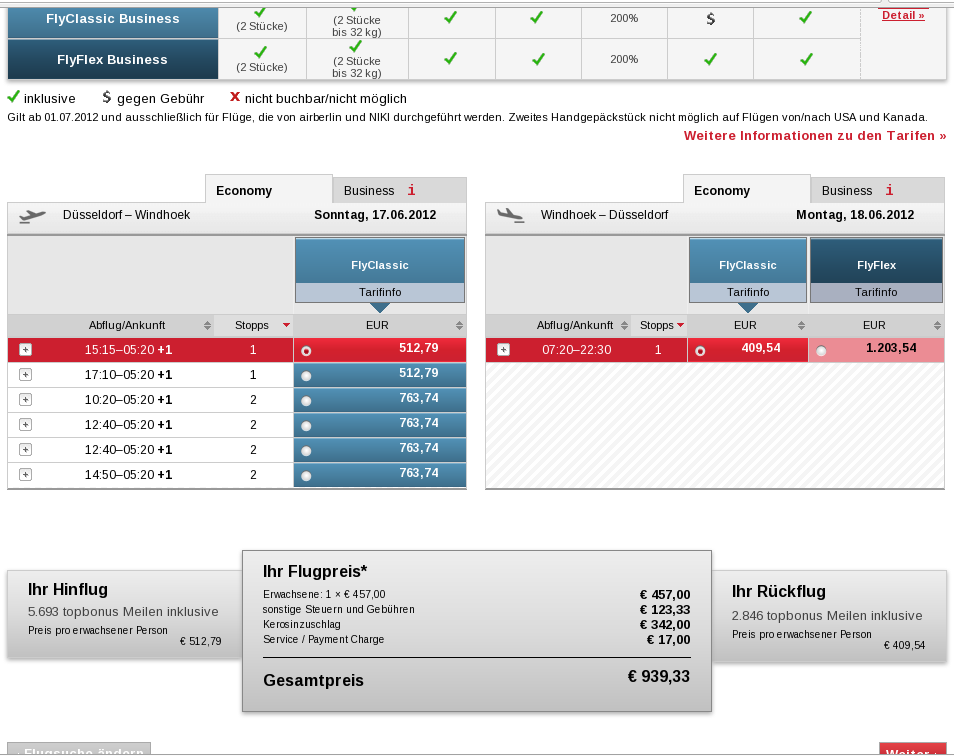
\includegraphics[scale=0.45]{Flug_Air_Berlin/Bildschirmfoto_am_2012-06-13_14_47_22.png} 

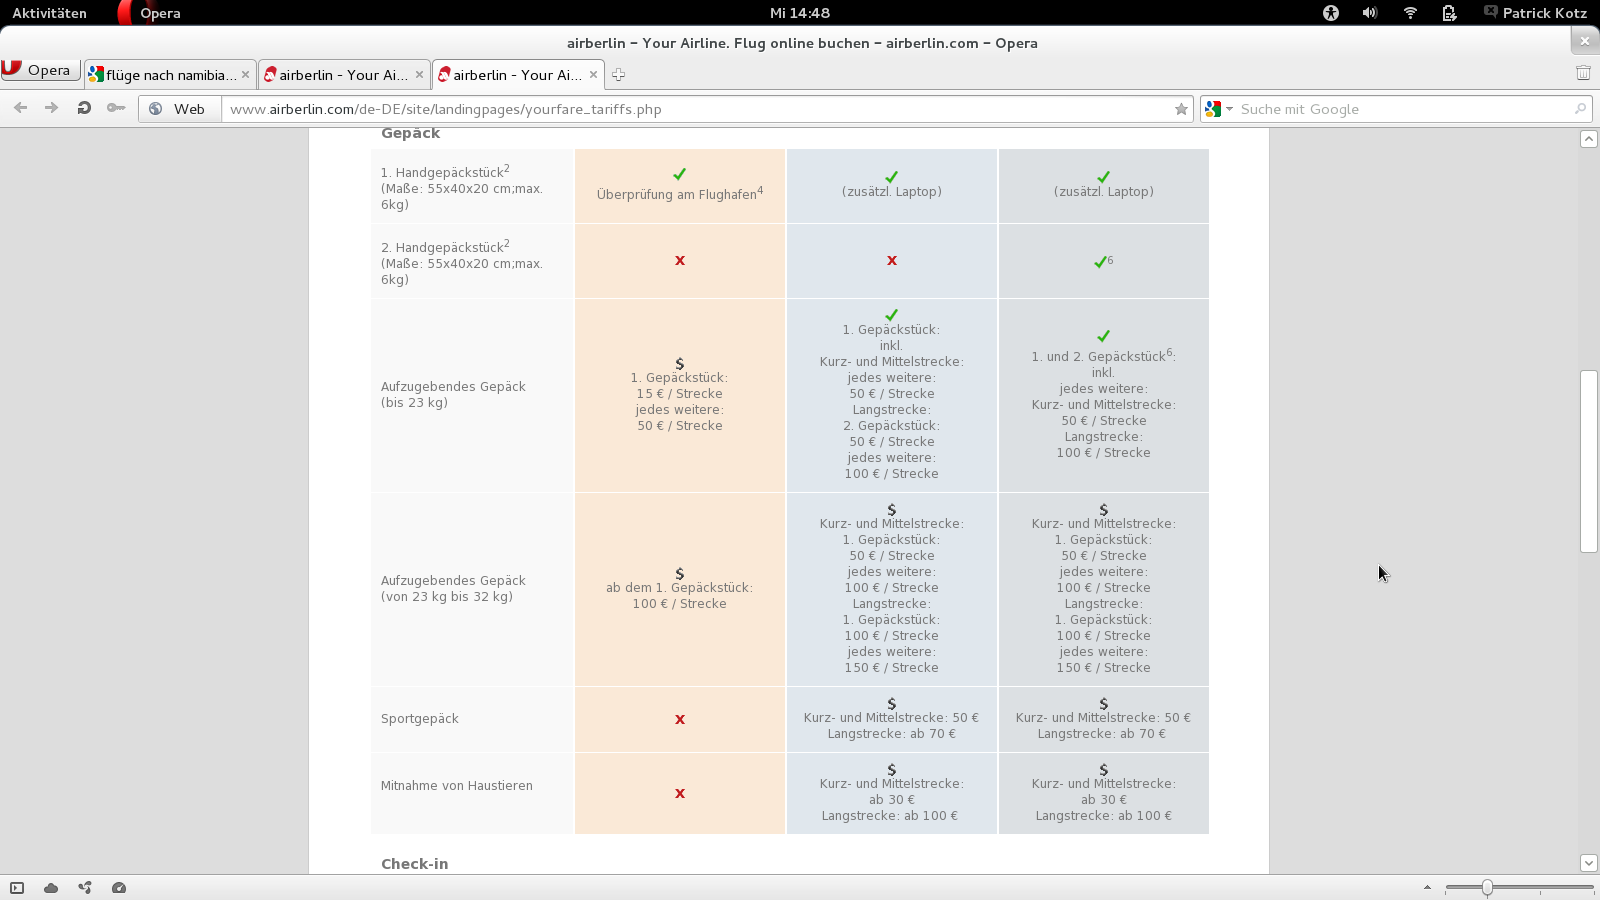
\includegraphics[scale=0.45]{Flug_Air_Berlin/Bildschirmfoto_am_2012-06-13_14_47_26.png} 

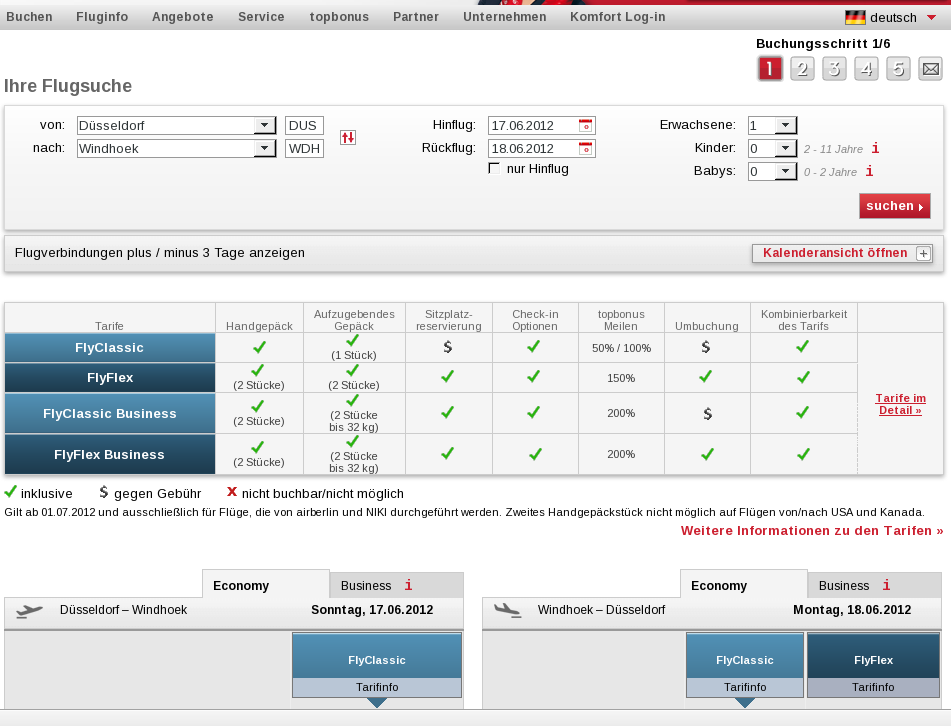
\includegraphics[scale=0.45]{Flug_Air_Berlin/Bildschirmfoto_am_2012-06-13_14_47_43.png} 

\end{document}
